\chapter{脱線せずに話せるようになる 3-2-1 スピーキング術!}

ここでは、きわめて実際的な問いから始める。突然その場で答えを求められたとき、どうすれば頭をより速く働かせられるのか。Zhang は、抽象的な意味での自信をもっと持てとか、気持ちを鼓舞する助言によって答えたりはしない。まず失敗の型から入り、話が崩れ始める地点を切り出し、それから、圧力のかかった場面でもすぐ手に取れるごく小さな枠組みを導入する。したがってこの講義は、制御された議論として展開される。混乱を診断し、混乱を構造へ置き換え、その構造を生きた例で試すのである。

\section{冒頭の問題}

講義は一つの問いで始まる。誰かに何かを尋ねられ、こちらに準備ができていないとき、何が起こるのか。答えは、単に緊張するというだけではない。思考があまりに速く枝分かれしてしまうのである。頭の中に多すぎる方向が開き、そのどれか一つが選ばれ、安定する前に、話し始めてしまう。これらのノートの言い方を借りれば、冒頭の因果連鎖は
\begin{equation}
\text{準備のできていない問い}
\;\Rightarrow\;
\text{焦った探索}
\;\Rightarrow\;
\text{とりとめのない話}.
\end{equation}
ということになる。これが、この講義における最初の本当の構造である。話が散漫になることは原初的な問題そのものではない。それは、探索過程のより深い乱れが目に見える形で現れた結果なのである。

Zhang はすぐに、この診断に重みを与えるため、それを自分自身のこととして語る。彼自身、以前はそうしていたのだという。彼の描写によれば、その結果は単なる言葉の乱雑さではなく、自信の崩落である。私たちは自分を無能に感じ、実際以上に自信がなさそうに見え、そのやりとり全体が苛立たしく、あるいは気まずいものになってしまう。ここが重要なのは、この講義が本当のところ巧みな言い回しについての話ではないからである。問題は、言葉が構造を追い越してしまうとき、何が起こるかにある。

\subsection{質問 \& 答え}

\paragraph{質問。} なぜ、その場で答えを求められると話がとりとめなくなるのか。

\paragraph{答え。} 思考がまだ整理の線を見つけていないうちに、発話が始まってしまうからである。Zhang の比喩では、脳内で ``十数個のブラウザタブ'' が開く。まさに的確な像である。候補となる方向が一度に多すぎるほど現れ、そのうち一つを選んでそこから組み立てる代わりに、探索のただ中で話し始めてしまう。したがって、話の散漫さは、気質の問題である以上に、構造の失敗なのである。

\section{焦りから頼れる型へ}

この乱れを診断してからはじめて、Zhang は解決へと向きを変える。彼は、準備された内容と即興で話すことを対比する。内容に準備があるときには自信は高まり、即興を強いられるときには自信は下がる。そこで彼は決定的な問いを発する。準備がないとき、私たちは何に立ち戻るのか。

彼の答えは率直である。たいてい、私たちは散漫な話し方へと立ち戻ってしまう。ここで講義の主要な対象が必要となる。フレームワークは飾りとして導入されるのではない。非常時の退避機構として導入されるのである。
\begin{equation}
\text{フレームワークがない}
\;\Rightarrow\;
\text{散漫さへと立ち戻る},
\qquad
\text{フレームワーク}
\;\Rightarrow\;
\text{構造へと立ち戻る}.
\end{equation}
この式が、この章の蝶番である。いったんこれが見えれば、残りの講義は自然に続いてゆく。問題は、言葉が足りないことではない。問題は、圧力のかかった場面で、すぐに取り出せる小さな構造を持っていないことなのだ。

Zhang は短く会場に問いかける。ふだんからコミュニケーションにフレームワークを使っている人はどれくらいいるか。その確認の目的は、統計的な精密さにあるのではない。教育的な対比にある。ほとんどの人は、意識しては使っていない。そこで講義は、ことさらに単純な一つを導入する。

\section{\texorpdfstring{$3,2,1$}{3,2,1} フレームワーク}

Zhang は、その意味を説明する前に、まずフレームワークの名を告げる。だからこそ、冒頭の板書が重要なのである。講義は、まず \((3,2,1)\) を一つの対象として提示し、そのあとでその意味を展開する。

\begin{figure}[h]
\centering

\includegraphics[width=0.72\textwidth]{lecture_13_figure_01.png}
\caption{冒頭の板書: \((3,2,1)\) が明示的にフレームワークとして導入されている。}
\end{figure}

板書のラベルは、最小限で率直である。
\begin{equation}
\left(3,2,1\right),
\qquad
\left[\text{フレームワーク}\right].
\end{equation}
これはまだ導出ではない。告知である。のちに操作的に使うことのできる、名を持った対象がここで与えられているのだ。

\begin{figure}[h]
\centering
\begin{tikzpicture}[x=1cm,y=1cm]
\node at (0,1.45) {$\left(3,2,1\right)$};
\draw[thick,rounded corners] (-2.1,0.25) rectangle (2.1,0.95);
\node at (0,0.60) {フレームワーク};
\end{tikzpicture}
\caption{冒頭の板書ラベルの最小限の再構成。}
\end{figure}

ついで Zhang は、この定義を口頭で繰り返す。そしてその反復が重要である。``three, two, one って何か。three steps, two types, and the one thing だ。'' さらに彼はもう一度言う。``Three steps, two types, one thing.'' この固定された順序は保っておくべきである。
\begin{equation}
3\ \text{つのステップ},\ 2\ \text{つのタイプ},\ 1\ \text{つのこと}.
\end{equation}

\begin{definition}
話題 \(T\) に対して、この講義の足場は、編集上は次のように表せる。
\begin{equation}
F_{321}(T)
=
\bigl(
\text{\(T\) のための3つのステップ},\;
\text{\(T\) の2つのタイプ},\;
\text{\(T\) についての1つのこと}
\bigr).
\end{equation}
この記法は、ノートを分かりやすくするために導入したものである。Zhang 自身が板書しているわけではない。
\end{definition}

だが同時に、Zhang はきわめて重要な実践的補足を行う。フレームワークの名は \(3,2,1\) の順で与えられているが、必ずしも最初の欄から入る必要はない。思考が最も引っかかりやすいところから始めればよいのである。
\begin{equation}
\text{entry}(F_{321}(T))
\in
\left\{
\text{\(T\) についての1つのこと},\;
\text{\(T\) の2つのタイプ/やり方},\;
\text{\(T\) のための3つのステップ}
\right\}.
\end{equation}
だからこそ、このフレームワークは圧力の中でも使える。それは硬直した台本ではない。許された分解の仕方を集めた、小さなメニューなのである。

講義はまた、使い道によってこのフレームワークを動機づける。Zhang は、いまでも自分がこれを使っていること、この Q\&A のまさにいま使っていること、SNS のコンテンツづくりにも使っていること、そして準備時間がほとんどないときにはいつでも使っていることを述べる。これらの言葉は新しい記法を増やしはしないが、なぜこのフレームワークに注目する価値があるのかを説明している。それは教室の珍品ではなく、現に働いている道具なのだ。

\subsection{質問 \& 答え}

\paragraph{質問。} \(3,2,1\) とは、正確には何を意味するのか。

\paragraph{答え。} 講義の厳密な順序に従えば、それは three steps, two types, one thing である。だが、より深い要点は、これによって三つの小さな答えの型が与えられるということだ。話題全体を一度に探し回る代わりに、私たちは許された型の一つを選び、そこから始める。したがってこのフレームワークは、暗記するための標語ではなく、分解の仕方を凝縮した小さな族なのである。

\section{実演例: avocado}

フレームワークを定義すると、Zhang はただちにそれを試す。聴衆にランダムな話題を求め、返ってきたのが ``avocado'' である。ここは講義の重要な拍である。フレームワークは抽象の中にぶら下げられたままにはされない。任意の話題に対して、実地に耐えるかどうかが試される。

ワークショップ中の板書は、この足場を最も明瞭に視覚化している。

\begin{figure}[h]
\centering

\includegraphics[width=0.82\textwidth]{lecture_13_figure_03.png}
\caption{ワークショップの板書: 左の板書は \(3,2,1\) の足場を、右の板書は第二の段階的フレームワークを示している。}
\end{figure}

左の板書には、すでに口頭で述べられた構造がそのまま見えている。
\begin{equation}
3\ \text{つのステップ},\ 2\ \text{つのタイプ},\ 1\ \text{つのこと}.
\end{equation}
右の板書には、\(\#\text{Framework}\) という見出しの下に、別のフレームワークが示され、\(S_1,S_2,S_3,S_4\) という段階と下向きの方向づけが見て取れる。長い手書きの各段階ラベルは判読が確実でないため書き起こさないが、段階的な運動そのものは、慎重に保存するには十分明確である。
\begin{equation}
S_1 \to S_2 \to S_3 \to S_4.
\end{equation}
この右側の板書は、講義の主線に対しては副次的である。しかし視覚的には重要だ。Zhang が一つの小技だけでなく、フレームワークという類そのものの観点から考えていることを思い出させてくれるからである。

\begin{figure}[h]
\centering
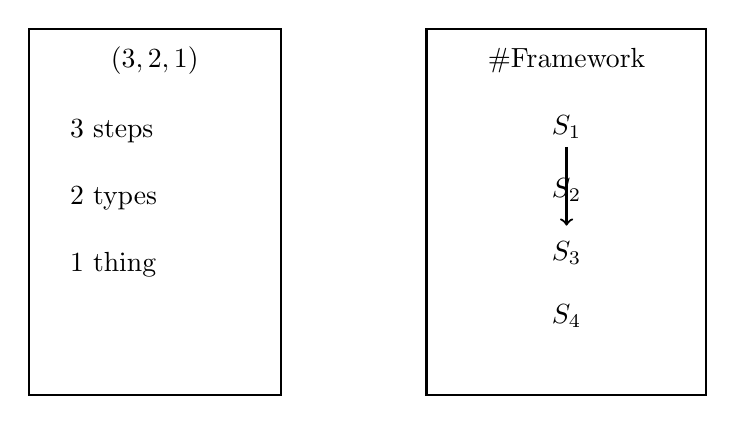
\begin{tikzpicture}[x=1cm,y=1cm]
\draw[thick] (-4.9,-0.2) rectangle (-1.7,4.45);
\node at (-3.3,4.05) {$\left(3,2,1\right)$};
\node[anchor=west] at (-4.5,3.15) {$3$ steps};
\node[anchor=west] at (-4.5,2.30) {$2$ types};
\node[anchor=west] at (-4.5,1.45) {$1$ thing};

\draw[thick] (0.15,-0.2) rectangle (3.7,4.45);
\node at (1.93,4.05) {\#Framework};
\node at (1.93,3.20) {$S_1$};
\node at (1.93,2.40) {$S_2$};
\node at (1.93,1.60) {$S_3$};
\node at (1.93,0.80) {$S_4$};
\draw[->,thick] (1.93,2.95) -- (1.93,1.95);
\end{tikzpicture}
\caption{見えている板書構造の整えた再構成。右側の板書の詳細ラベルは、確実に読めないため省いてある。}
\end{figure}

では、avocado の例を、実際に行われた順序で追ってみよう。Zhang は ``three steps'' からは始めない。最も入りやすい欄、すなわち one thing から始める。その意味で、講義は先に述べた柔軟性を自ら実演している。この例は簡潔には
\begin{equation}
F_{321}(\text{avocado})
=
\bigl(
\text{3つの準備のステップ},
\text{2つの食べ方},
\text{それについての1つのこと}
\bigr),
\end{equation}
と記録できるが、実際の運用では最後の成分から先に入っている。

実演の縮約は次のようになる。
\begin{align}
\text{1 thing} &:\ \text{彼にとって avocado は keto diet に非常に適している},\\
\text{2 ways} &:\ \text{つぶしてトーストにのせるか、果物のようにそのまま食べるか},\\
\text{3 steps} &:\ \text{切る、つぶす、味つけする}.
\end{align}
これが、この講義における、動きの中にあるフレームワークの最初の完全な実演である。

混乱との対比も同じく重要である。Zhang は、うまくいった道筋だけを見せるのではない。制御されていない代案も、わざと劇的に示す。フレームワークがなければ、頭は可能な筋道を次々と回ってしまう。色、熟れ具合、保存、レシピ、まだ食べられるかどうか、何を混ぜるべきか。略記すれば、
\begin{equation}
\text{avocado}
\;\Rightarrow\;
\{\text{緑},\text{熟れ具合},\text{保存},\text{レシピ},\ldots\}
\;\Rightarrow\;
\text{頭が真っ白になるか、舌がもつれる}.
\end{equation}
このフレームワークが機能するのは、探索を狭めるからである。話題空間全体を探し回る必要はない。いくつかの許された型のうち一つを選べばよいのである。

\subsection{質問 \& 答え}

\paragraph{質問。} このフレームワークは、どうやって脳に拠りどころを与えるのか。

\paragraph{答え。} その場で生きている選択肢の数を減らすからである。輪郭のない話題を前にして一度にあらゆる方向を探す代わりに、私たちはその話題を三つの小さな型のどれかへ圧縮する。one thing、two types、あるいは three steps である。すると頭は、やみくもに探すのではなく、組み立て始めることができる。

この例には、もう一つ微妙な補足がある。Zhang は局所的に ``two types'' を ``two ways'' へと緩めている。これは矛盾ではない。むしろそこが要点の一部である。第二の欄は、分類にも、小さな対比にも使えるだけの広さを持っている。これに対して第三の欄は、明確に手順的な分解を与える。したがって同じフレームワークが、記述的な話し方にも、順序的な話し方にも対応できるのである。

\section{圧力、間、そしてフレームワークの広い一族}

ここで講義は、次の緊張へと向かう。視聴者はこう思うはずである。なるほど、それは講師にはできた。だが自分にもできるのか。Zhang は、この反応を先回りして真正面から受け止める。答えは yes である。なぜなら、これから実際にそれをやるからだ。そう言って彼は一人の学生を前に呼び、話題を与える前に、圧力の一因になりそうなものを取り除く。三つすべてをやる必要はない。いちばん易しいものを一つ選べばよい、と。

この細部は落としてはならない。このフレームワークは、最大出力を求める要求ではない。許可の構造なのである。
\begin{equation}
\text{まず許された欄を一つ選ぶ}
\;\Rightarrow\;
\text{答えを安定させる}
\;\Rightarrow\;
\text{必要ならそこから広げる}.
\end{equation}
また、学生が自分はまだ準備できていないと認めたとき、彼は、誰だって準備万端ではないのだと言う。これもまた、精密な動機づけの一手である。講義は、圧力が消えるとは約束しない。圧力に対して、構造で向き合えると約束するのである。

この実践が終わる前に、講義は短く立ち止まり、\(3,2,1\) が、いくつもあるコミュニケーション・フレームワークのうちの一つにすぎないことを思い出させる。このより広い位置づけの視覚的証拠が、挿入された板書ショットである。

\begin{figure}[h]
\centering

\includegraphics[width=0.78\textwidth]{lecture_13_figure_04.png}
\caption{挿入された板書ショット: \(3,2,1\) の足場が、より広い見出しの下に置かれており、フレームワークのより大きな一族を示している。}
\end{figure}

ここで確かなのは、板書の階層であって、下部の宣伝的バナーではない。後者は脇に置く。上部に見えている構造は
\begin{equation}
\text{Visibility},
\qquad
2)\ \left(3,2,1\right).
\end{equation}
である。その下に、見慣れた足場が置かれ、色つきの接続線が右側の注記へと伸びているが、その正確な文言は確定しがたい。最も安全な読みは、\(3,2,1\) が、より広いコミュニケーション道具の一覧の中に位置づけられている、という程度のものである。

\begin{figure}[h]
\centering
\begin{tikzpicture}[x=1cm,y=1cm]
\node at (0,3.85) {Visibility};
\node at (0,2.95) {$2)\ \left(3,2,1\right)$};

\node[anchor=west] at (-1.85,1.95) {$3$ steps};
\node[anchor=west] at (-1.85,1.20) {$2$ types};
\node[anchor=west] at (-1.85,0.45) {$1$ thing};

\draw[->,thick] (0.75,1.95) -- (2.25,1.95);
\draw[->,thick] (0.75,1.20) -- (2.25,1.95);
\draw[->,thick] (0.75,0.45) -- (2.25,1.95);
\node at (3.4,1.95) {適用先?};
\end{tikzpicture}
\caption{見えている板書階層の慎重な再構成。右側の適用ラベルは、手書きが完全には確定できないため一般的に留めてある。}
\end{figure}

\subsection{質問 \& 答え}

\paragraph{質問。} 毎回、このフレームワークの三つすべてを使わなければならないのか。

\paragraph{答え。} いいえ。Zhang は、いちばん易しいものを選べばよいと明言している。これは些細な便宜ではない。圧力の下でこのフレームワークを使えるものにしている、実際上の規則そのものなのである。この足場は、始めるための手がかりであって、あらゆる場面で完全に埋めなければならない負担ではない。

\section{travel: 時間圧の中での転移}

ここでようやく、講義は自ら作り出した生の緊張を解く。ランダムな話題は ``travel'' である。Zhang は数え始める。three, two。学生は数え終わる前に答え始める。その素早さ自体が証明の一部である。フレームワークが、そのやりとりのテンポを変えてしまうほど速く、利用可能になったのである。

この応答を講義の構造順に書けば、
\begin{equation}
F_{321}(\text{travel})
=
\bigl(
\text{計画する、予約する、行く},
\text{国内/地域旅行か、海外旅行か},
\text{travel はすばらしい}
\bigr).
\end{equation}
となる。学生が実際に行った順に書けば、操作上の系列は
\begin{align}
\text{1 thing} &:\ \text{travel はすばらしい。行きたいところへどこへでも行ける},\\
\text{2 types} &:\ \text{国内・地域の travel と、international travel},\\
\text{3 steps} &:\ \text{計画する、予約する、行く}.
\end{align}
となる。これが転移の試験であり、そして転移は成功している。

講義はそのあと、解釈へと戻る。フレームワークがなければ、Zhang の言うように、脳はまた混乱へと回り始めるだろう。travel って何のこと、私は travel は嫌い、子どもたちを煩わせたくない、等々。このフレームワークは、まさにその崩れを防ぐ。だが Zhang の最後の要点は、言葉の整頓以上のところにある。彼は、学生のボディランゲージに注目する。彼女はマイクのほうへ身を乗り出し、その課題へ向かって前に出た。だからこそ、この講義の結びの構造は
\begin{equation}
\text{フレームワーク}
\;\Rightarrow\;
\text{即応できる感じ}
\;\Rightarrow\;
\text{自信あるコミュニケーション}.
\end{equation}
と書かれるべきなのである。フレームワークは、文を変えるだけではない。その文がどんな姿勢から発せられるかをも変えるのである。

\subsection{質問 \& 答え}

\paragraph{質問。} なぜフレームワークは、何を言うかだけでなく、どれだけ準備ができていると感じるかまで変えるのか。

\paragraph{答え。} いったん安定した答えの型が利用可能になれば、発話はもはや混沌への跳躍には感じられなくなるからである。フレームワークは、最初の一文が発せられる前に、不確実性を減らしてくれる。その認知的な縮減が、身体の準備として目に見えるようになる。話し手は一歩前へ出て、身を乗り出し、ためらいを少なくして伝えられるようになるのである。

\section{まとめ}

この講義は、きわめて明快な順序で展開される。まず、失敗の診断。準備のない問いは焦った探索を生み、焦った探索はとりとめのない話を生む。次に、欠けていた対象を同定する。すなわち、立ち戻るためのフレームワークである。ついで、その中でもとりわけ小さく有用なものとして、\((3,2,1)\) を導入する。three steps, two types, one thing である。そのあとで、任意の話題に対してこのフレームワークを実演し、それが制御不能な枝分かれをどう抑えるかを示し、最後に、生の時間圧のかかった練習の中で、その転移を確かめる。

最後に残るのは、簡潔なスピーキングの算法である。開かれた話題に直面したとき、私たちは領域全体を探し回らない。話題を小さな許容形へと縮約し、最も取っかかりやすいところから始め、そこから外へ向かって組み立てる。ここでの数学的内容は軽い。だが構造は確かにある。フレームワークとは、思考が発話に間に合うように到着させる方法なのである。